\section{Challenges for Partitioning with Enclaves}
\label{sec:background}
In this section, we will give a brief overview of \sgx{}, and discuss 
the key challenges developers face when trying to manually partition applications using a technology such as \sgx{}.
%discuss the programming models and threats to security of \sgx{} enclaves.

\subsection{Background on \intel{} SGX Enclaves}

\intel{} \sgx{} ({\it Software Guard Extension})
is a set of new x86/x64 instructions
introduced in the \intel{} Skylake processor family.
Using \sgx{}, an 
application can designate part of its virtual memory as an {\em enclave}.
The CPU guarantees that the contents of the enclave never leave the CPU package unencrypted.
The CPU also measures the integrity of a binary loaded into the enclave, and offers remote attestation,
similar to a TPM\fixmedp{cite}.

%%% create a protected memory region, called an {\em enclave}, inside it's virtual memory,
%%% where it can load its security sensitive data with hardware-enforced isolation from the untrusted OS. 
%%% The processor with \sgx{}
%%% guarantees that any data loaded in enclave
%%% stays encrypted in the DRAM, by using a secret key deterministically derived from the application's cryptographic measurement and the CPU secret. 

\sgx{} is an appealing tool for protecting small amounts of highly-sensitive data or code, because it can defend 
against a malicious or compromsed OS, hypervisor, or even hardware peripheral.
For instance, \fixmedp{Foo} et al.~\fixmedp{cite that SGX workshop paper} show how SGX can be used
to build a trusted path from a video chat application to a GPU and network card, which maintains confidentiality and integrity of the
video stream, even if the OS is compromised.
Simlarly, because DRAM contents are encrypted, SGX can resist cold-boot attacks~\cite{halderman09coldboot} or 
malicious peripheral devices~\cite{hudson15thunderstrike}.


%%% \sgx{} also proves the integrity of loaded binaries to remote trusted entities
%%% using mutual attestation based on a symmetric key generated from the measurements of communicating entities.
%%% \sgx{} usage model mostly involve the launched enclave mutually attesting the trusted host
%%% to obtain provisioning of security-sensitive information
%%% through a trusted channel. Such an execution model leverages resources such as CPU and DRAM from vulnerable untrusted \sgx{}-enabled hosts owned by cloud providers
%%% by extending the trust from
%%% the hosts owned and trusted by the clients or service providers.
%%% For instance, \sgx{} can isolate the decoder engine in an enclave
%%% after authenticating the customers to enforce Digital Right Management (DRM) even if the digital data is hosted on an untrusted cloud server.

%Use cases of \sgx{} mostly involve the launched enclave
%retrieving a cryptographically signed attestation from the processor,
%to exchange security critical information with remote servers through secured channels.
%The effect is equivalent to expanding the trusted space from remote servers
%to the local end, to harness local resources such as CPU and DRAM.

%One must note that \sgx{} only promises the integrity of application binaries
%initially loaded in enclaves.
%The gap between integrity of binaries and complete security has to be filled
%by ones who develop and approve the applications.
%More specifically, the clients are responsible of
%testing whether the applications contain any vulnerabilities
%that lead to information leak.
%To minimize the risk of leaving any flaws in the applications unintentionally,
%developers often tend to cut down the trusted computing base (TCB)
%of the applications. With smaller TCB, clients who launched the enclaves
%can more easily reason about the thoroughness of securing the execution.

%%% The key strength of \sgx{} enclaves over other software-based isolation framework such as
%%% {\em Flicker}, {\em Inktag} or {\em Virtual Ghost} is
%%% the ability to defend against attacks at the hardware level.
%%% These software-based solution often
%%% rely on a hypervisor below the OS to isolate the applications.
%%% If the hardware is attacked,
%%% the attackers may still bypass the software checkpoints,
%%% or directly steal confidential information from the DRAM.
%%% For \sgx{}, the only hardware included in the TCB is the CPU package,
%%% and in practice CPUs are believed to be hard to attack.
%%% Using techniques like cold-boot attacks~\cite{halderman09coldboot}
%%% to peek into DRAM content,
%%% or intruding the boot process using corrupted peripheral devices like Thuderstrike~\cite{hudson15thunderstrike}
%%% will affect any software-based isolation, but not \sgx{} enclaves.

\paragraph{Non-Partitioned Applications.}
One approach to using SGX is to run an entire application in the enclave.
This is exemplified by Haven~\cite{baumann14haven}, which runs a Windows application and all supporting libraries
on top of a {\em library OS}.  This approach is illustrated on the left side of Figure~\ref{fig:libosvssdk}.
The library OS approach does not require any application changes, but bloats the TCB \fixmedp{Rough number of how big Haven is}.
By pulling millions of lines of extraneous code into an enclave, there is a significantly increased risk 
of vulnerabilities that disclose
sensitive data, such as Heartbleed~\fixmedp{cite}.
The library OS approach is useful in its simplicity of deployment and can provide practical benefits, 
such as protecting an application from an untrusted cloud hypervisor.

\begin{figure}[t!]
\centering
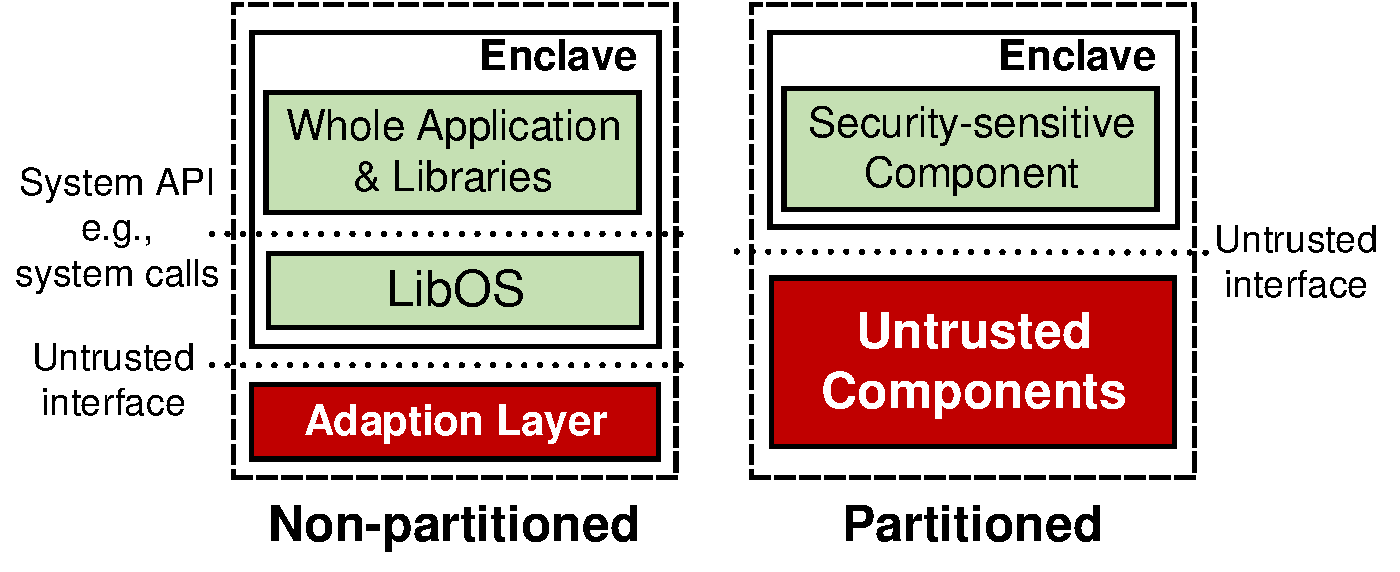
\includegraphics[width=\linewidth]{figures/libosvssdk.pdf}
\footnotesize
\vspace{-0.2in}
\caption{
Comparison between the libOS-based model (e.g., Haven)
and the partitioned model for programing applications in enclaves.
Green (light) boxes are trusted components and red (dark) boxes are untrusted.
The libOS-based model yields a larger TCB in the enclave,
while the partitioned model requires developers to be responsible for determining the untrusted interface at the enclave boundary.
}
\label{fig:libosvssdk}
\end{figure}


This paper focuses on a second usage model for enclaves, where the application is partitioned into
untrusted and one or more trusted components (right side of Figure~\ref{fig:libosvssdk}).
Sensitive data and computation are placed inside of enclaves.  This approach requires the developer to
identify sensitive code and data; design and harden an interface between trusted and untrusted components; 
modify the application source; and reason about potential information flows at the enclave boundary.
This effort can be non-trivial and subtle, but for application developers motivated by interests such as 
regulatory compliance or competitive advantage in business, the additional effort can yield a much smaller trusted computing
base (TCB), and thus a reduced attack surface.
A key goal of \sysname{} is to minimize the developer's effort to partition an application---both in lines of 
code changed, and in leveraging language analysis to reason about narrow points in the application's data and control flow.


%To achieve smaller TCB, the software development kit of \sgx{}
%intends to encourage developers to partition the applications and
%keep only security sensitive components in the enclaves.
%Such an intention is exactly contradicted by the trust model of \haven{},
%which must trust the loaded application as a whole.
%Except for the cases in which the whole applications must be secured,
%\haven{} actually downgrades the trustworthiness of enclaves.
%Figure~\ref{fig:libosvssdk} shows the comparison of the two models.

%%% In prior works using \sgx{} enclaves to secure applications,
%%% developers choose between two different programing models: the {\em library-OS-based} and the {\em partitioned} model (as shown in Figure~\ref{fig:libosvssdk}).
%%% In the libOS-based model, developers run the whole standalone,
%%% legacy application inside the enclave, using library OS such as {\em Haven} or {\em Graphene libOS} to facilitate the rich OS features.
%%% The main benefit of using library OS is that developers only have to employ minimal efforts to port any existing application.
%%% Even when designing new applications, developers bear no responsibility
%%% of identifying and reasoning about
%%% the security sensitive part of the application.

%%% However, when using libOS-based model, a sophisticated legacy application
%%% will yield huge trusted computing base (TCB) in the enclave,
%%% aggravating the risk of leaking information through vulnerabilities inside the enclave.
%%% Known bugs such as {\em the heart-bleeding bug} has shown that
%%% running security sensitive code like an encryption engine, and management code such as heart-beating service in the same address space
%%% can cause vulnerabilities that compromise the security by leaking the encryption key.
%%% As a result, using a partitioned model, developers can isolate only the most security sensitive components in an enclave,
%%% and leave the remaining code outside to minimize the TCB.

%%% Developers have to define the {\em untrusted interface} 
%%% to allow parts of a partitioned applications to interact.
%%% The untrusted interface is used either by the the untrusted components
%%% to trigger execution of the isolated components,
%%% or by isolated components to use untrusted rich OS features, such as networking for provisioning and sending the execution output to the remote hosts.
%%% Unlike the libOS approach that has a fixed untrusted interface (for different applications) at their interaction boundary with the OS,
%%% the width of untrusted interface for a partitioned application is up to developers' design.
%%% The \intel{} SDK for \sgx{} supports a set of syntaxes to specify the type and direction of flow for parameters of the untrusted interface, and enforces primitive
%%% type-checking of incoming values on transition to enclave.

%%% The trade-off between the libOS-based and partition model is based 
%%% on ease of development, the width of untrusted interface,
%%% and size of TCB.
%%% The benefit of the libOS-based model is that developers can save the effort
%%% of determining what to execute in the enclave,
%%% and whether the execution is safe,
%%% because the whole application is wrapped in the enclave.
%%% However, the risk of having vulnerabilities in the applications
%%% is not reduced, but in fact amplified due to the addition of
%%% the library OS (e.g., the Haven binary yields around a few hundred MBs) to TCB.
%%% On the other hand, if the developers are willing to spend effort on carefully identifying the untrusted interface and re-designing their application around this interface, the partitioned model can improve security guarantees by minimizing the attack vectors.

%%% The goal of \sysname{} is to provide the benefits of both models.
%%% \sysname{} support a partitioned model
%%% for developers to isolate security-sensitive part of a \java{} application in enclave,
%%% and provide a language-based tool to automatically partition
%%% the minimal supporting classes to generate the enclave image.
%%% Even in the case where the isolated component need to frequently interact with the untrusted component or the OS,
%%% the language protection technique of information flow tracking
%%% guarantees that the secrets in the enclave are never leaked
%%% without the developers explicit consent. 

\paragraph{Side Channels and Denial-of-Service.}
In the current \sgx{} design, side channels are a signficant concern for either the library OS or partitioned model, and are out of the scope of this paper.
A controlled channel attack~\fixmedp{cite} can single step enclave execution by inducing page faults
in the enclave.  \sysname{} does not specifically defend against side channel attacks,
and we expect that any solution to this problem involves redesigning the division of labor in virtual
memory management for enclaves.

Similarly, there is no guarantee that a compromised application will ever enter
an enclave.  Denial-of-service attacks are out of scope for this paper.


\subsection{Challenges for Application Partitioning on SGX}

\sgx{} provides useful building blocks for secure applications, but does not
absolve the programmer of any responsibility for reasoning about end-to-end security.
Bugs in the application or supporting libraries can still disclose sensitive data from an enclave,
and porting code into SGX can be subtle.
This subsection outlines several pitfalls in partitioning an application for SGX.

%%% \sgx{} enclaves provide strong isolation guarantee for applications,
%%% against the malicious or vulnerable application components, system stack,
%%% and hardware (except the CPU itself).
%%% However, the security guarantees of the \sgx{} enclave is dependent on whether the developers design perfect applications without exploitable vulnerabilities that may compromise the application's security.
%%% As the application developers are not perfect,
%%% even applications or components isolated in enclave can face threats to their security.
%%% As follows, we discuss a few potential threats
%%% to the enclave security,
%%% even under the assumption that the SGX hardware is implemented as completely secure --- which can be another threat otherwise. 

%\fixmedp{I roughly want the rest of this section to have a problem, explanation, solution structure, with the overall theme being that this is subtle and we really need some analysis tools to get this right}

\paragraph{Writes outside of the enclave.}
SGX allows code inside the enclave to read and write data structures 
outside of the enclave.  Thus, it is easy for a developer to inadvertently write
code that discloses a secret, say by using a library that memoizes intermediate results to the untrusted heap.
A fundamental requirement is that developers must be able to reason about (or assert)
what code can and can't access data {\em outside} of the enclave.
\fixmedp{Can we say anything about whether such tools exist before Civet?}

%\fixmedp{Do I recall correctly that you can easily write to data outside of the enclave?  If so, this seems like something easy to get wrong, especially 
%if a library memoizes intermediate results.  The developer needs to be able to tell 
%Unless I am full of shit, can we paragraph-ize this fixme?

\paragraph{Application vulnerabilities.} 
The major source of threats to enclave security is any internal vulnerabilities in the isolated components,
such as buffer overflows and other memory corruption attacks.
Moreover, although \sgx{} code integrity guarantees make enclaves resistant to code injection,
an attacker may still manipulate control flow using code-reuse attacks~\cite{code-reuse-attacks}.
Moreover, recent research ~\cite{hudata} show that even with perfect control flow integrity,
attackers can still manipulate the execution to leak the secrets through information flow.

Fundamentally, this argues for some combination of static analysis
and runtime monitoring of 
enclave code.  This is greatly simplified when the enclave code is written in higher-level languages
with properties 
%amenable to analysis.
%with type safety, memory safety, and other 
%that provide important 
%safety properties,
such as type safety or memory safety. %, thereby reducing the likelihood of these vulnerabilities.
Ideally, one would formally verify security properties of enclave code~\cite{moat}; this verification is significantly aided by using 
higher-level languages amenable to formal reasoning.
%Verification is significantly harder
%with C or x86 assembly.

%% \paragraph{Applications are not perfect} 
%% The \sgx{} hardware cannot prevent applications from copying secrets out of the enclave without limiting functionality.
%% The trusted isolated components can copy any sensitive data from the enclave to the unencrypted memory, and potentially leak the enclave secrets.
%% The primary risk in the isolated components
%% is often memory corruption vulnerabilities, such as buffer overflow,
%% %Because in enclave applications can access any part of out-of-enclave memory unrestrictedly,
%% prevalent in applications that are not implemented in type-safe languages.

%% The best known technique to prevent vulnerabilities is to model the applications and verify them using {\em formal verification}.
%% While Sinha et.al.,~\cite{moat} use formal verification to prove confidentiality of enclave programs, it is impractical to accurately model complex sophisticated applications.
%% As a result, in addition to formal verification, maintaining smallest TCB
%% in the isolated components is the most practical approach 
%% to ensure enclave security,
%% and is the main reason to choose partitioned programming model over
%% libOS-based model.


\begin{figure}[t!]
\centering
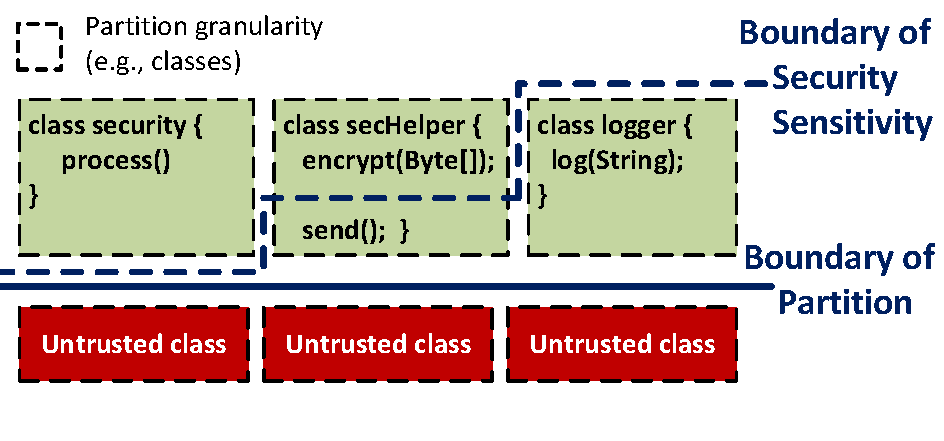
\includegraphics[width=\linewidth]{figures/partition.pdf}
\footnotesize
\vspace{-0.3in}
\caption{
Partitioning --- either manually or by automated tool ---
often causes wider boundary of partition than the actual security sensitivity boundary
due to (a) design granularity : {\tt secHelper} contains a {\tt send()} method that is not partitioned from the rest of the class by design.
The reasons of having the gap vary, for instance, 
that is less security sensitive, but due to the granularity it is not partitioned from the rest of the class or (b) better performance :  the less security sensitive {\tt logger} class is kept in the privileged level to service frequent method calls.
}
\label{fig:partition}
\end{figure}

%However, even if developers partition the applications and run only
%security sensitive components in the enclave,
%the developers may still leave some code irrelevant to
%enclave secrets inside the enclave.
%The reasons of having more-than-minimal TCB in enclaves
%are often that developers have to partition code in the granularity of source files or functions,
%or developers have to import more code to limit the width of interface and
%the frequency of interaction with the untrusted code.

\paragraph{Identifying ``pinch points''.}
Reasoning about where in a program to draw the line between 
trusted and untrusted code is subtle.
On one hand, the developer has an incentive to minimize the size of the 
API between the enclave and untrusted code, as well as an incentive to
minimize the total code in the enclave.  These goals can sometimes be at odds.
Each entry and exit to an enclave has a cost roughly comparable to a
process context switch\fixmedp{right?}; an easy way to reduce enclave entries and exits is to simply 
pull more code into the enclave, which increases the size of the TCB.

\fixmedp{I'm not sure how to explain Figure~\ref{fig:partition}, but it needs an explanation.}

Fundamentally, the art of paritioning an application is to find a ``pinch point'' or
``narrow waist'' in the application, where there is a natural point to insert an API and 
security checks.  This is indeed as much art as science, often done manually by experts\fixmedp{any more supporting evidence or cites?}.
It is unlikely that the average developer will successfully navigate this design process without analysis tools, such as \fixmedp{examples?},
to help identify these natural division points.


%% Experts can use a manual partitioning technique to achieve smallest TCB for the isolated components compared to automated tools.
%% However, the manual partitioning costs a lot of effort,
%% and rare expertise, lack of which can cause larger TCB.

%% Neither manual nor automated partitioning is perfect:
%% the resulted boundary of partitioning often has a gap from the actual boundary of security sensitivity (as shown in figure~\ref{fig:partition}),
%% leaving more code in the privileged level
%% than what's actually needed.
%% Having the gap between the ideal and resulted boundary
%% is mostly inevitable, due to multiple reasons.
%% One common reason is the granularity of partitioning,
%% which can vary from a binary file, a component, a source file,
%% a class, a method (a function) to a line of code.
%% Another reason is that a component or a method may be too frequently called
%% by the security sensitive code,
%% laying the boundary between the component or method from the security sensitive side may bring too much overhead or risk,
%% because the execution crosses the boundary too often.
%% Therefore, developers often will balance among the effort of partitioning,
%% risk or cost of communicating between different partitions,
%% and minimizing the TCB in the security sensitive parts.

\fixmedp{Maybe move the commented paragraph below down into the design section?  I'd like to downplay the plugs for our work here, and instead fulfill these promises later}
%% \sysname{} automates partitioning of applications,
%% based on the boundary at the classes which the developers marked
%% as the interfaces of the enclave.
%% Only the classes that are depended by the marked classes
%% will be included in the enclaves,
%% to minimize the TCB.
%% Although not all classes pulled into the enclaves
%% are necessarily security sensitive,
%% the enclaves are protected from the potential vulnerabilities in those classes,
%% by the security guarantees of \java{} language,
%% and the information flow tracking in \sysname{}.

%Another threat to \sgx{} is the vulnerability of the 
%security sensitive code running in the Enclave. The 
%main guarantee of \sgx{} to isolate the secure data 
%from other components and privileged OS is undermined 
%if the Enclave code can be tricked to leak the 
%security sensitive data to the attacker. Executing 
%buggy code in \sgx{} enclave can inadvertently leak 
%information if the attacker can exploit memory-safety 
%vulnerabilities like buffer overflow and dangling 
%pointers.  

% Cumbersome and approximation to partition code
%The developers have to manually partition their code 
%into security sensitive and insensitive part. If this 
%partitioning is done by a novice developer, some of 
%the security insensitive parts of the application can 
%end up in the security sensitive part, increasing the 
%Trusted Computing Base(TCB). Moreover, the 
%partitioning of code is not straightforward, which 
%can also contribute to a less stricter TCB. The bigger the TCB, the more %vulnerable is the Enclave code to attacks.

% Buggy Code leads to inadvertant information leakage


% SGX code only Integrity protected not confidential
%Moreover, \sgx{} only protects the integrity of the enclave code. The security critical part of the application is stored in plaintext while the secret data is provisioned securely after attestation. However, \sgx{} does not protect the confidentiality of enclave application code which may be executing a secret algorithm. \fixmebj{Talk more about the problem motivating security tag preservation.}
%\sgx{} can natively guarantee either code integrity or
%code confidentiality (as part of the enclave data), but not both.
%If application code is included in the enclave measurement and
%verified by the hardware,
%the code must stay in plaintext as part of the enclave image.
%If any code is stored or provisioned in encrypted forms,
%the application or infrastructure in enclave must dynamically load
%the code after decryption.
%Supporting dynamic loading makes enclaves open to code injection
%if the applications have exploitable vulnerabilities.

\paragraph{Code Integrity {\em and} Confidentiality.} 
The hardware-level \sgx{} code integrity mechanism is based on a cryptographic
signature of a static binary in plaintext.
If any application dynamically loads any code after the enclave's initial measurement,
the initial application must be trusted to attest the loaded code.
The subtle tension is that there is no way to protect the confidentiality of
a secret algorithm, except by dynamically loading an encrypted binary.
Dynamically loading code increases the risk of code injection attacks and other control flow compromises.

Any application partitioning solution that protects sensitive algorithms
must have a robust dynamic loader that can measure encrypted libraries or classes.
\sysname{} includes a loader that can measure encrypted class files,
provisioned from a trusted host.

%% \sgx{} enclaves require code integrity in the isolated applications.
%% If the code integrity is not maintained, adversaries can corrupt the enclave code to
%% force the applications to leak the information provisioned from the remote,
%% trusted hosts.
%% \sgx{} hardware only guarantees
%% the integrity of the code initially loaded into the enclaves.
%% However, if an application choose to dynamically
%% load any code after the enclave starts,
%% the application is responsible for the integrity of the code loaded.
%% The fact that dynamic loading of applications, libraries or components
%% is a feature that can potentially make enclaves vulnerable and open to code injection,
%% raises concerns against supporting managed languages in the enclaves.

%% On the other hand, code confidentiality can be a desirable feature,
%% for application developers who prefer keeping the secret sauce of their algorithms concealed.
%% To enable the feature of code confidentiality in enclaves, the protected code must be dynamically loaded into the enclave,
%% because the \sgx{} hardware only accept
%% the initial loaded code to be in plaintext.
%% \sysname{} provides both code integrity and confidentiality by verifying
%% every classes dynamically loaded into the enclaves,
%% and allows loading classes provisioned from trusted hosts.


%% In general \sgx{} enclaves are prone to having side channels, such as timing channels. Because \sgx{} relies on the untrusted OS for paging,
%% an enclave will always leak page fault addresses, except the lower 12 bits (offsets in pages).
%% Such a leakage gives the untrusted OS to amplify the side channels,
%% by forcing page faults on every instruction or memory access.
%% This so-called {\em Controlled Channel Attack} is common to all applications who use \sgx{} protection, regardless of the programming models.
%% \sysname{} does not specifically defend against side channel attacks.

%% \paragraph{Denial-Of-Service Attacks}
%% \sgx{} is not designed to be safe against denial-of-service attacks.
%% Because the untrusted OS still controls the host resources,
%% there are countless ways to prevent an enclave from making progress.
%% For example, the OS can simply starve the enclaves by
%% never scheduling CPU, memory or other resources to the enclaves.
%% \sysname{} does not specifically defend against denial-of-service attacks.

\paragraph{Discussion.}  This
section has outlined several pitfalls for developers of partitioned applications.
These common pitfalls render the hardware protections of SGX useless.
Language-level analysis can automate error-prone reasoning in the best case, or, in the worst case, 
can at least offer invaluable guidance to the developer.  For SGX-style
hardware to be useful to a wide array of developers, developers need language-level
tools that can also factor in hardware-level protection mechanisms.



%- Motivate the problem.
%- List all attack vectors
%- How can JAVA help?



















































































